\documentclass[main.tex]{subfiles}

\newcommand{\LeptonInjector}{\texttt{LeptonInjector}}
\newcommand{\LeptonWeighter}{\texttt{LeptonWeighter}}
\newcommand{\NuGen}{\texttt{NuGen}}
\newcommand{\ANIS}{\texttt{ANIS}}
\newcommand{\Python}{\texttt{Python }}
\newcommand{\MCEq}{\texttt{MCE{\scriptsize Q}}}
\newcommand{\MMC}{\texttt{MMC}}
\newcommand{\PROPOSAL}{\texttt{PROPOSAL}}
\newcommand{\CORSIKA}{\texttt{CORSIKA}}
\newcommand{\MUONGUN}{\texttt{MuonGun}}
\newcommand{\PHOTOSPLINE}{\texttt{Photospline}}
\newcommand{\boost}{\texttt{Boost}}
\newcommand{\hdf}{\texttt{HDF5}}
\newcommand{\boostpython}{\texttt{boost-python}}
\newcommand{\nusim}{\texttt{NUSIM}}

\newcommand\pythonstyle{\lstset{
    language=Python,
    basicstyle=\footnotesize,
    otherkeywords={self},             % Add keywords here
    keywordstyle=\color{deepblue},
    emph={MyClass,__init__},          % Custom highlighting
    emphstyle=\color{deepred},    % Custom highlighting style
    stringstyle=\color{deepgreen},
    %frame=tb,                         % Any extra options here
    showstringspaces=false            % 
}}

% Python for external files
\newcommand{\pythonexternal}[2][]{{
\pythonstyle
\lstinputlisting[#1]{#2}}}


% Python for inline
\newcommand\pythoninline[1]{{\pythonstyle\lstinline!#1!}}



% Cowan_2011
\begin{document}

\section{\LeptonInjector{} Event Structure~\label{sec:li_event}}

All \LeptonInjector{} events from a single process are saved to a single \hdf~file. Each \textbf{Injector} used in the generation process is given its own dataset inside the \hdf~file with four lists containing an entry for each event generated. Two lists are stored for the two final state particles' parameters, a third list contains the initial state particles' parameters, and a fourth list contains overall parameters for the events.
Each of the event-entries in each of the three lists of particles contain, in order: a number differentiating whether it is initial or final state, the particles' PDG ID~\cite{PhysRevD.98.030001}, the particles' positions, the particles' directions in radians, and the particles' energies. 
The overall properties stored for each event are shown in Figure~\ref{fig:tiks_struct}.
The impact parameter and total column depth are defined in Section~\ref{sec:injection} and shown graphically in Figures~\ref{fig:lepton_ranged2} and~\ref{fig:lepton_ranged4}.

\begin{figure*}[htb!]
\centering
\begin{tikzpicture}[
  grow via three points={one child at (0.5,-0.7) and
  two children at (0.5,-0.7) and (0.5,-1.4)},
  edge from parent path={(\tikzparentnode.south) |- (\tikzchildnode.west)}]
  \node {MC Events}
    % !!!: The names listed here do not appear to match the code
    child { node [selected] {\ttf properties}
        child { node [label=right:{energy of the interacting neutrino. [$\si\GeV$]}] {\ttf totalEnergy}}	
        child { node [label=right:{initial zenith of the lepton. [$\si\radian$]}] {\ttf Zenith}}
        child { node [label=right:{initial azimuth of the lepton. [$\si\radian$]}] {\ttf Azimuth}}
        child { node [label=right:{Bjorken $x$ of the interaction. [dimensionless]}] {\ttf finalStateX }}	
        child { node [label=right:{Bjorken $y$ of the interaction. [dimensionless]}] {\ttf finalStateY}}
        child { node [label=right:{Code of first final state particle. [dimensionless]}] {\ttf finalType1}}
        child { node [label=right:{Code of second final state particle. [dimensionless]}] {\ttf finalType2}}
        child { node [label=right:{Code of parent particle. [dimensionless]}] {\ttf initalType}}
        child {node {\ttf Ranged/Volume Quantities}
            child { node [label=right:{sampled distance from PCA to origin [$\si\cm$]}] {\ttf impactParameter}}
            child { node [label=right:{column depth considered for interaction. [$\si{\g\per\square\cm}$]}] {\ttf totalColumnDepth}}
            child [missing] {}
            child { node [label=right:{distance above the xy-plane [$\si\cm$]}] {\ttf z}}
            child { node [label=right:{distance from the z-axis [$\si\cm$]}] {\ttf radius}}
        }
    }
    child [missing] {}				
    child [missing] {}				
    child [missing] {}
    child [missing] {}			
    child [missing] {}	
    child [missing] {}
    child [missing] {}
    child [missing] {}
    child [missing] {}
    child [missing] {}
    child [missing] {}
    child [missing] {}	
    child [missing] {}
    child [missing] {}
    child [missing] {}
    child { node [label=right:{Event flux-less weight. [$\si{\GeV\square\cm\steradian}$]}] {\ttf LeptonInjectorWeight} } 
    ;
\end{tikzpicture}
%\internallinenumbers
\caption{Lepton Injector Monte Carlo event structure.}\label{fig:tiks_struct}
\end{figure*}

\section{LIC File Structure~\label{sec:lic_structure}}

Data serialized in the LIC file is written little-endian, regardless of machine architecture. 
When a LIC file is first opened, the \textbf{Controller} either overwrites any existing file with the same destination name or begins appending to the end of such an existing file. 
This behavior follows according to user-specification. 
If a new file is being written or an existing one overwritten, a block is first written to the file enumerating all \LeptonInjector{} particle types. 
A header is first written specifying the size of the block, the name of the enumeration, and the length of the enumeration. 
Then the name and number of each entry in the particle enumeration is written. 

Afterwards, each time a new \textbf{Generator} is prepared, the \textbf{Controller} writes a new block to the LIC file. 
Each of these blocks is prefaced with a header specifying the size of the block, the name of the block, and the version of the \LeptonInjector{} serialization code used to write the block. 
Then, all relevant generation parameters are written to the block. 
\section{Earth Model Density\label{sec:earthdensity}}

\LeptonInjector{} uses a modified Preliminary Reference Earth Model (PREM) for column depth calculations around the injection region. The density profile of which is shown in Figure~\ref{fig:earth_density}.

\begin{figure}[th!]
    \centering
    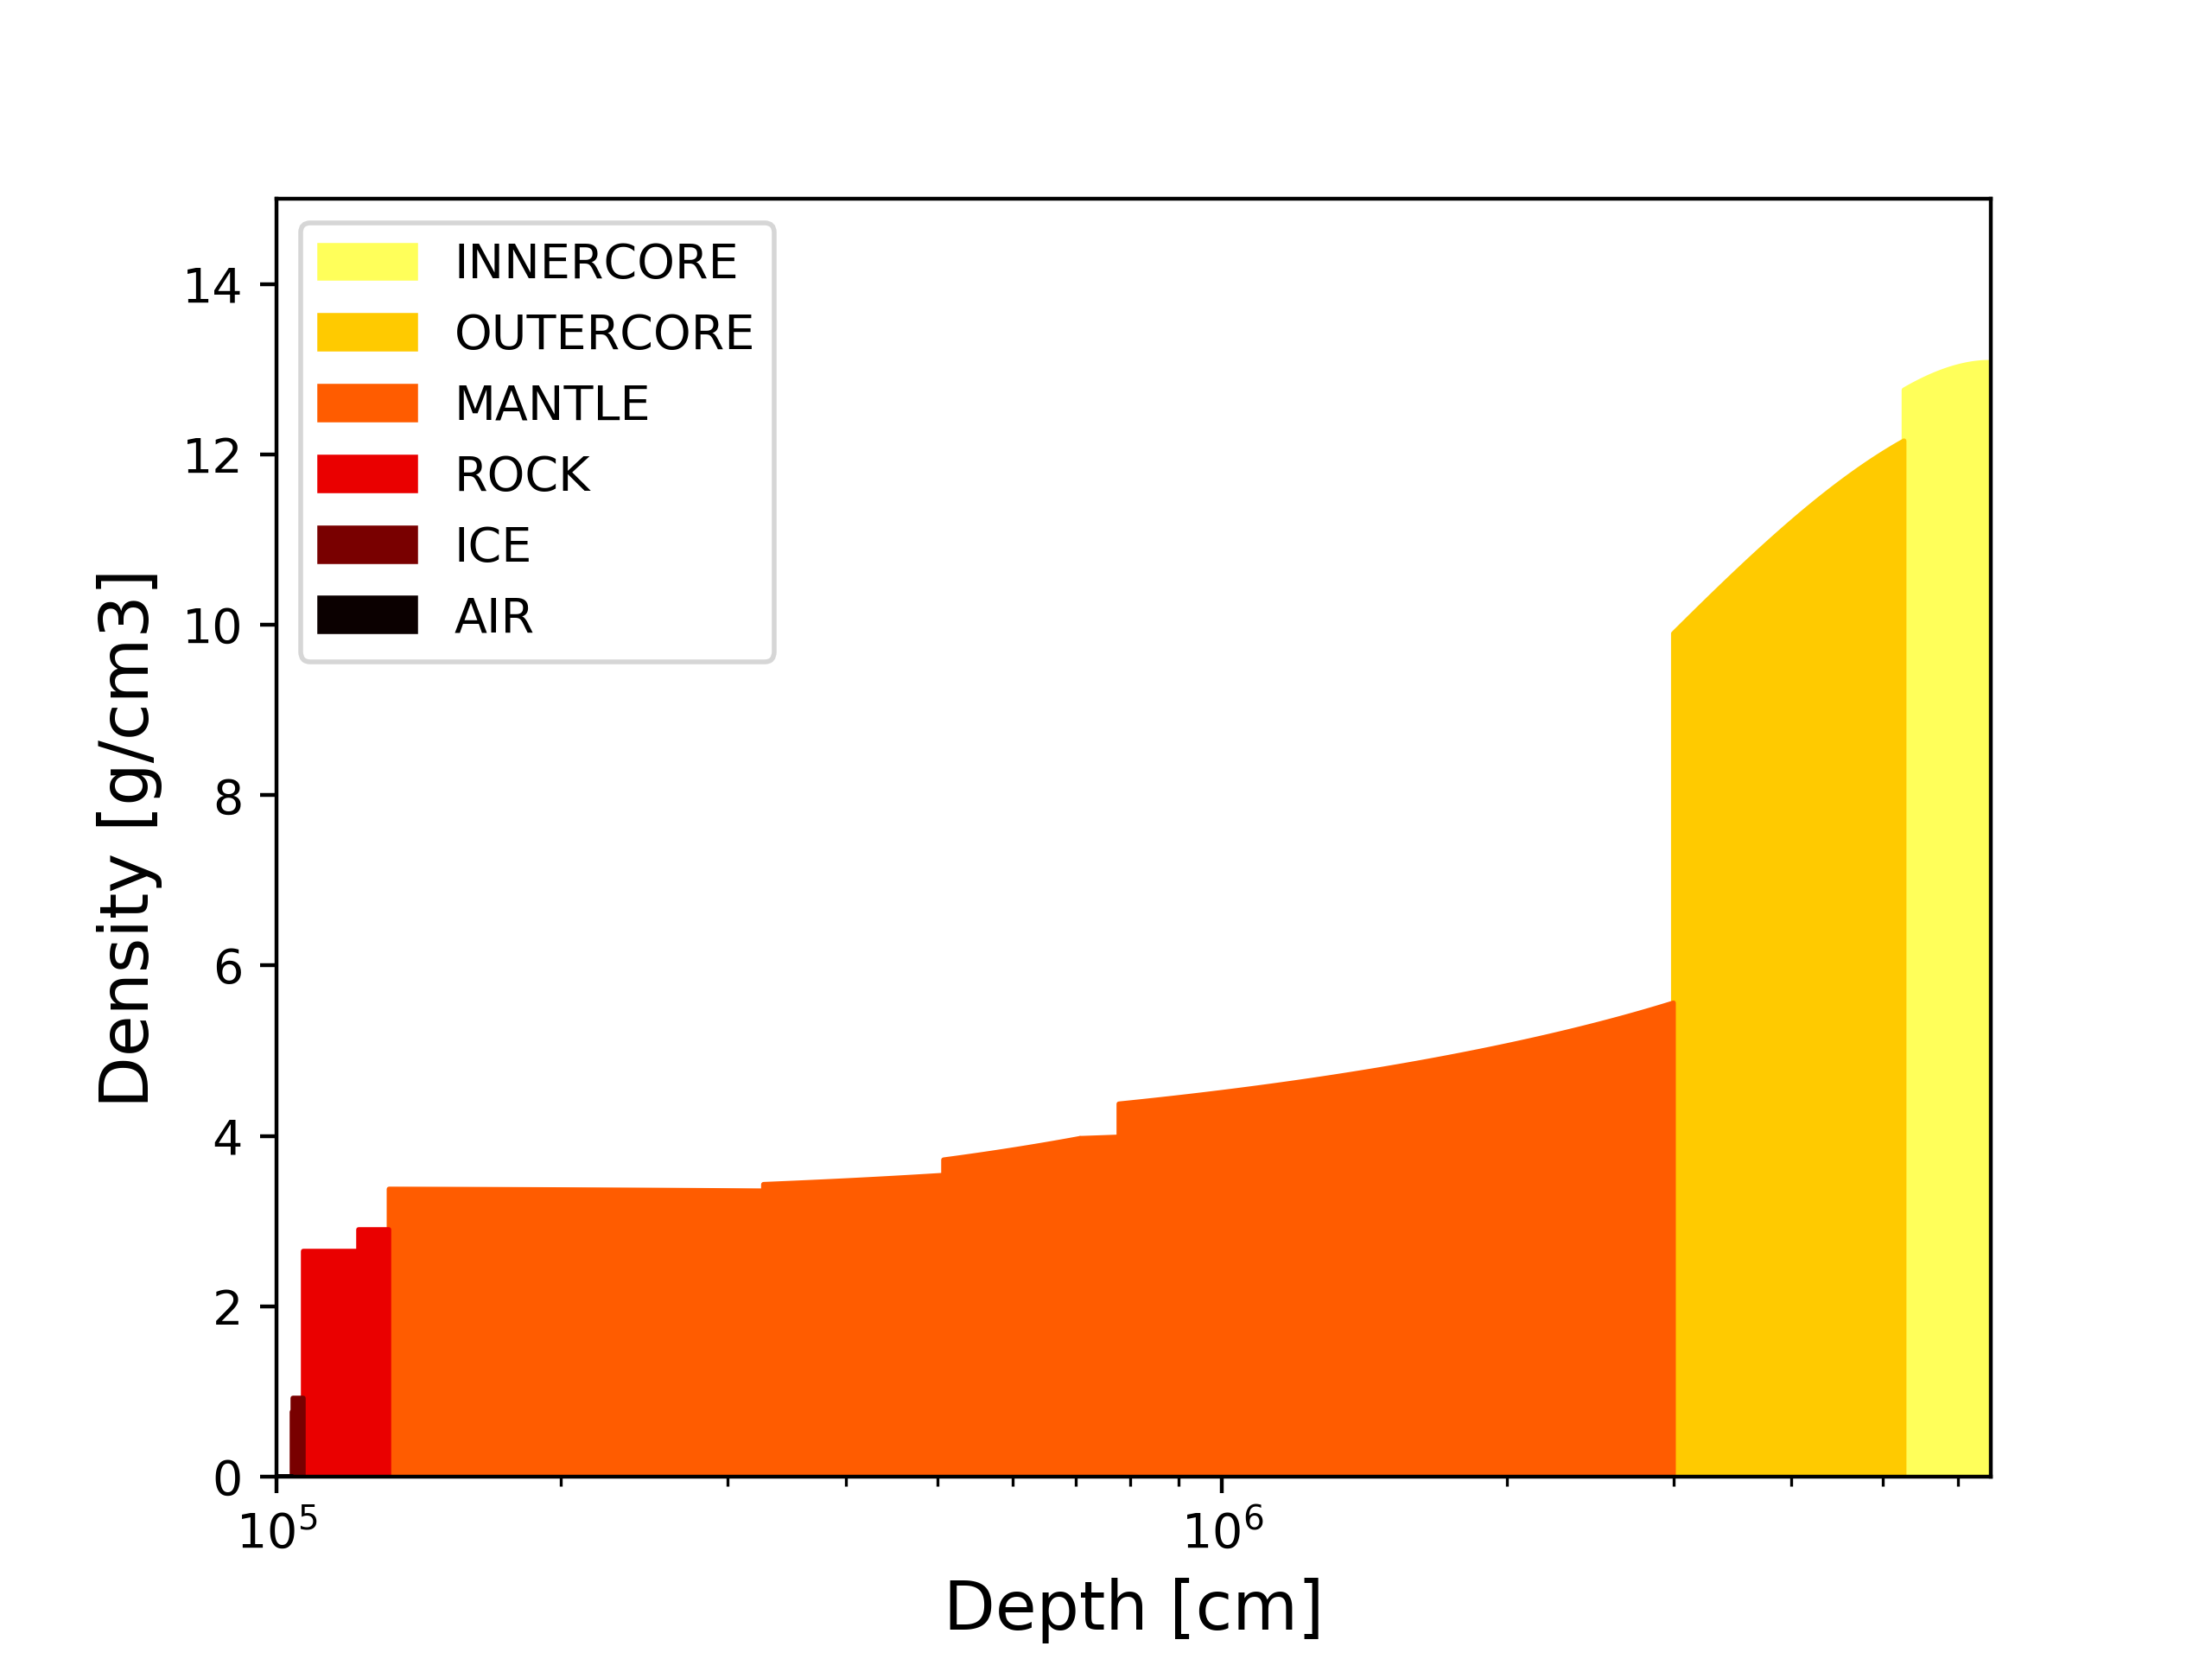
\includegraphics[width=0.8\linewidth]{figures/earth_density.png}
    \caption{The density of the \LeptonInjector{} Earth model as a function of depth from the edge of Earth's atmosphere.}
    \label{fig:earth_density}
\end{figure}

\section{Weighting}\label{sec:weight_append}

The generation procedure produces a set of neutrino properties that include the position, direction, energy, neutrino type, interaction type, and final state kinematic properties.
The distribution of these properties at generation may differ from those we would expect in a physical scenario, so the weighting procedure is designed to correct for these differences.
Beyond the distribution differences, weighting also corrects for differences in dimensionality and raw numbers of events.
In our prototypical scenario, the weight of an event is dimensionless so only a correction factor to the total number of events is needed ($N_\textrm{physical}/N_\textrm{gen}$).

In the case of ranged injection we can separate the generation probability density of an event into several independent components
\begin{equation}
p_\textrm{gen} = p_\textrm{gen}^\textrm{neutrino type} \times p_\textrm{gen}^\textrm{interaction type} \times p_\textrm{gen}^\textrm{energy} \times p_\textrm{gen}^\textrm{direction} \times p_\textrm{gen}^\textrm{impact} \times p_\textrm{gen}^\textrm{depth} \times p_\textrm{gen}^\textrm{kinematics}.
\end{equation}
The generators in \LeptonInjector{} only deal with one neutrino and interaction type each, so $p_\textrm{gen}^\textrm{neutrino type}$ and $p_\textrm{gen}^\textrm{interaction type}$ will either be one or zero depending on if the event matches what can be produced by the generator.
Similarly, $p_\textrm{gen}^\textrm{energy}$ is the probability distribution of injected neutrino energies which is zero for events with neutrino energies outside the bounds of the generator.
Directions are distributed uniformly in ranged injection and so $p_\textrm{gen}^\textrm{direction} = 1/\Omega_\textrm{gen}$ where $\Omega_\textrm{gen}$ is the total solid angle available to the generator.
The $p_\textrm{gen}^\textrm{impact}$ term is the probability distribution related to the impact parameter and angle; since events are sampled uniformly on a disk, this term is the inverse of the disk area, $p_\textrm{gen}^\textrm{impact} = 1/A_\textrm{gen}$, for events intersecting the disk and zero otherwise.
Events are sampled uniformly with respect to column depth along the considered line segment, so the positional distribution of events can be described as $p_\textrm{gen}^\textrm{depth} = \rho_\textrm{gen}(\ell)/X_\textrm{gen}^\textrm{col}$, where $\rho_\textrm{gen}(\ell)$ is the local target mass density where the event is injected and $X_\textrm{gen}^\textrm{col}$ is the total column depth of targets along the considered line segment.
Finally, $p_\textrm{gen}^\textrm{kinematics}$ is the probability distribution of the events kinematic variables; for charged current and neutral current events this is $p_\textrm{gen}^\textrm{kinematics} = (\partial_{xy}\sigma_\textrm{gen}^{\textrm{tot}, i}) / (\sigma_\textrm{gen}^{\textrm{tot}, i})$.

These terms in the generation probability must then be paired with their physical counterparts.
Since our hypothesis can specify the number of neutrinos per type, the neutrino type can be neglected beyond this number correction and the $p_\textrm{gen}^\textrm{neutrino type}$ term from the generator.
The energy, direction, and impact terms all have their counterpart in the neutrino flux $\Phi_\textrm{physical}$, which specifies the physical neutrino distribution in energy, direction, area, and time.
The flux, when paired with a detector livetime $L_\textrm{physical}$ also specifies the total number of neutrinos $N_\textrm{physical}$ by the relation
\begin{equation}
L_\textrm{physical} \times \Phi_\textrm{physical} = N_\textrm{physical} \times p_\textrm{physical}^\textrm{neutrino type} \times p_\textrm{physical}^\textrm{energy} \times p_\textrm{physical}^\textrm{direction} \times p_\textrm{physical}^\textrm{impact}.
\end{equation}

The remaining terms, $p_\textrm{gen}^\textrm{interaction type}$, $p_\textrm{gen}^\textrm{depth}$, and $p_\textrm{gen}^\textrm{kinematics}$, deal with the neutrino interaction itself, which requires special care.
The generation process assumes that the neutrino interacts within a certain region and with a specific interaction type.
In reality, neutrinos on a path to the detector are potentially subject to any of several different interactions, and may pass through the Earth entirely unimpeded.
Thus, we need to account for the probability that the neutrino in the physical scenario would interact within the region considered by the generator $p_\textrm{physical}^\textrm{interaction}$, the depth distribution of all neutrino interactions within that region $p_\textrm{physical}^\textrm{depth}$, the probability that a specific interaction occurs once the interaction point has been chosen $p_\textrm{physical}^\textrm{interaction type}$, and finally the kinematic distribution $p_\textrm{physical}^\textrm{kinematics}$.
The former two terms, $p_\textrm{physical}^\textrm{interaction}$ and $p_\textrm{physical}^\textrm{depth}$ depend explicitly on the line segment considered by the generator when choosing the neutrino interaction vertex.
The interaction probability can be cast in terms of the ``survival'' probability, $p_\textrm{physical}^\textrm{interaction} = 1-p_\textrm{physical}^\textrm{survival}$, the probability that the neutrino will pass through the region without interacting.
The survival probability is given by
\begin{equation}
p_\textrm{physical}^\textrm{survival} = \exp\left(-{\int_{\ell_i}^{\ell_f}{d\ell \sum_{p,i} n_\textrm{physical}^p(\ell) \sigma_\textrm{physical}^{\textrm{tot},p,i} }}\right),
\end{equation}
where $p$ iterates over the possible targets (usually nucleons and electrons), $i$ iterates over interaction types, and $n_\textrm{physical}^p(\ell)$ is the density of target $p$ at a point $\ell$ along the considered line segment
Thus,
\begin{equation}
p_\textrm{physical}^\textrm{interaction} = 1-\exp\left(-{\int_{\ell_i}^{\ell_f}{d\ell \sum_{p,i} n_\textrm{physical}^p(\ell) \sigma_\textrm{physical}^{\textrm{tot},p,i} }}\right).
\end{equation}
Another way of writing this is in terms of the total column depth for each target $X_\textrm{physical}^{\textrm{col}, p}$, target molar mass $M_p$, and Avagadro's number $N_A$, such that
\begin{equation}
p_\textrm{physical}^\textrm{interaction} = 1-\exp\left(-N_A{\sum_{p,i} (X_\textrm{physical}^{\textrm{col}, p}/M_p) \sigma_\textrm{physical}^{\textrm{tot},p,i} }\right).
\end{equation}
The implementation in \LeptonWeighter{} groups protons and neutrons together and assumes that the molar mass of nucleons is $\SI{1}{\gram\per\mol}$.
The depth distribution $p_\textrm{physical}^\textrm{depth}$ follows a similar form as the survival probability, but is normalized within the generation bounds such that
\begin{equation}\begin{split}
p_\textrm{physical}^\textrm{depth} &= \exp\left(-{\int_{\ell_i}^{\ell}{d\ell \sum_{p,i} n_\textrm{physical}^p(\ell) \sigma_\textrm{physical}^{\textrm{tot},p,i} }}\right) \\
& \hspace{1cm} / \int_{\ell_i}^{\ell_f}{d\ell}\exp\left(-{\int_{\ell_i}^{\ell}{d\ell \sum_{p,i} n_\textrm{physical}^p(\ell) \sigma_\textrm{physical}^{\textrm{tot},p,i} }}\right),
\end{split}\end{equation}
which can similarly be recast in terms of the density or column depth.
The last two terms, $p_\textrm{physical}^\textrm{interaction type}$ and $p_\textrm{physical}^\textrm{kinematics}$, depend only on the position and type of the interaction, and so are independent of the generator.
Once we assume that an interaction occurs at a known location, the probability of a specific interaction $p_\textrm{physical}^\textrm{interaction type}$ is the ratio of total cross sections at that location $p_\textrm{physical}^\textrm{interaction type} = (\sigma_\textrm{physical}^{\textrm{tot}, i})/(\sum_j \sigma_\textrm{physical}^{\textrm{tot}, j})$ where the subscript $j$ iterates over all possible interactions.
For the chosen interaction type, the kinematic distribution is simply $p_\textrm{physical}^\textrm{kinematics} = (\partial_{xy}\sigma_\textrm{physical}^{\textrm{tot}, i}) / (\sigma_\textrm{physical}^{\textrm{tot}, i})$ in the case of charged or neutral current interactions.

By pairing up the terms we can see all the effects that are accounted for in the event weight
\begin{equation}
w_\textrm{MC} = \frac{N_\textrm{physical}}{N_\textrm{gen}} p_\textrm{physical}^\textrm{interaction} \frac{p_\textrm{physical}^\textrm{neutrino type}}{p_\textrm{gen}^\textrm{neutrino type}} \frac{p_\textrm{physical}^\textrm{interaction type}}{p_\textrm{gen}^\textrm{interaction type}} \frac{p_\textrm{physical}^\textrm{energy}}{p_\textrm{gen}^\textrm{energy}} \frac{p_\textrm{physical}^\textrm{direction}}{p_\textrm{gen}^\textrm{direction}} \frac{p_\textrm{physical}^\textrm{impact}}{p_\textrm{gen}^\textrm{impact}} \frac{p_\textrm{physical}^\textrm{depth}}{p_\textrm{gen}^\textrm{depth}} \frac{p_\textrm{physical}^\textrm{kinematics}}{p_\textrm{gen}^\textrm{kinematics}}.
\end{equation}
Practical implementations of this replace some of the physical terms with the flux and livetime to obtain the event weight
\begin{equation}
w_\textrm{MC} = \frac{L_\textrm{physical}\Phi_\textrm{physical}}{N_\textrm{gen} p_\textrm{gen}^\textrm{neutrino type} p_\textrm{gen}^\textrm{energy} p_\textrm{gen}^\textrm{direction} p_\textrm{gen}^\textrm{impact}} \times p_\textrm{physical}^\textrm{interaction} \times \frac{p_\textrm{physical}^\textrm{interaction type}}{p_\textrm{gen}^\textrm{interaction type}} \times \frac{p_\textrm{physical}^\textrm{depth}}{p_\textrm{gen}^\textrm{depth}} \times \frac{p_\textrm{physical}^\textrm{kinematics}}{p_\textrm{gen}^\textrm{kinematics}}.
\end{equation}

When simulation is created using multiple generators we must consider the probability that a particular event may be generated in either generator, regardless of which generator it originated from.
The behavior we desire is such that events from non-overlapping regions of the parameter space retain their original single-generator weights, but events that reside in the overlap regions are down-weighted to account for the overlap.
The event weight then takes the form
\begin{equation}
w_\textmd{MC} = \left[\sum_i \left(p_\textmd{physical}^{i}\right)^{-1} \times p_\textmd{gen}^{i}\right]^{-1},
\end{equation}
where the superscript $i$ denotes the different generators, $p_\textmd{physical}^{i}$ is the physical contribution to the weighting, and $p_\textmd{gen}^{i}$ is the generation contribution to the weighting.
Note the superscript $i$ on the physical contribution is there because the terms $p_\textrm{physical}^\textrm{interaction}$ and $p_\textrm{physical}^\textrm{depth}$ depend on the particular generator.
If the generation settings governing the line segment along which the event is injected are common to all generators then this dependence can be dropped and $p_\textrm{physical}$ can be factored out.

The above description in the weighting starts from the ranged injection procedure, but only minor modifications are needed for this to be applicable to volume injection.
The difference arises from the $p_\textrm{gen}^\textrm{depth}$ and $p_\textrm{gen}^\textrm{impact}$ terms on the generation side and $p_\textrm{physical}^\textrm{depth}$ and $p_\textrm{physical}^\textrm{interaction}$ on the physical side.
These generation terms are directly analogous to steps in the ranged injection procedure where the position of closest approach and interaction vertex position are chosen.
In the volume injection, the interaction vertex is chosen in a single step, so we can replace these two generation terms with the single $p_\textrm{gen}^\textrm{position}$ term which is a uniform probability density along the line segment within the injection cylinder and zero outside.
The physical terms only differ in that the line segment considered for the calculation now must come from the volume injection procedure.
Specifically, the line segment considered passes through the interaction vertex following the injected neutrino direction, beginning and ending at the boundaries of the injection cylinder.

These differences between the ranged and volume injection mean that the physical contributions to the weighting will differ between the two, and must be calculated separately for each event if both methods are used in the event generation.

Finally, the approximation used in Eq.~\ref{eq:approx_weight} can be obtained by expanding the depth and interaction terms for a vanishing product of the interaction cross section and column depth.
For the column depths and cross sections used in \LeptonInjector{}, this approximation remains valid for sub $\si\ZeV$ neutrino energies.

\section{Code Examples}

\subsection{Generation Example\label{sec:example_generation}}

This \Python example is included in the \LeptonInjector{} source code.
It creates an Injector in Ranged mode for producing CC muon-neutrino events of initial energy between $\SI{1000}\GeV$ to $\SI{100000}\GeV$, and outputs the data to an \hdf~file.

\pythonexternal{examples/inject_example.py}


\subsection{Weighting Example\label{sec:example_weighting}}

The following \Python example is included in \LeptonWeighter{}.
It reads a set of generated events and computes the weights of for a given neutrino cross-sections and fluxes.
The result is stored in an HDF5 file for later usage.

\pythonexternal{./examples/weighting_example_python.py}


\end{document}